\titledquestion{Sangaku}

Sangakus är en typ av japanska (ofta geometriska) matematikproblem som under Edo perioden lämnades vid tempel som en form av offergåva\footnote{Om detta faktiskt gjordes som en form av religiös dyrkan, eller för att skryta och visa alla andra tempelbesökare vilka svåra problem man lyckats lösa är inte helt klar.}.

En av de kändaste har att göra med tre cirklar som alla tangerar varandra och en linje.
\begin{figure}[H]
    \centering
    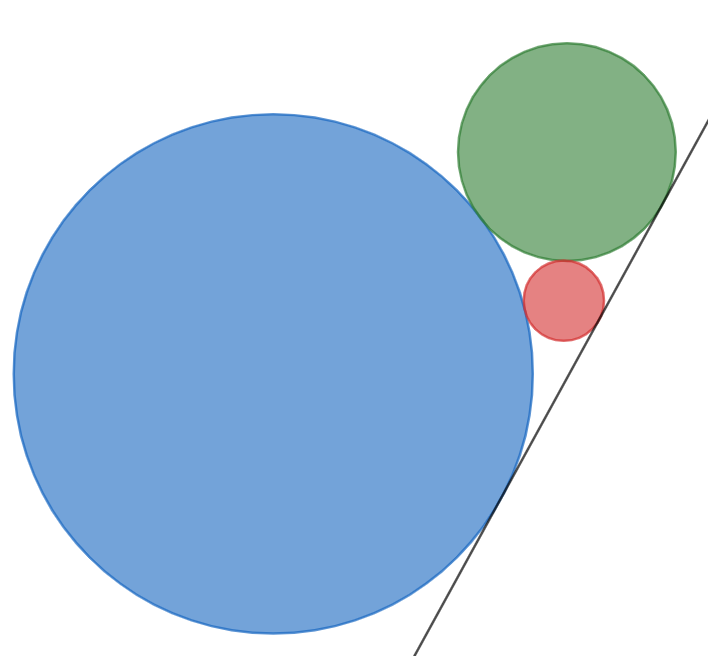
\includegraphics[width=0.5\linewidth]{img/tre cirklar.png}
    \caption{Tre cirklar som alla tangerar en linje.}
\end{figure}


Radien av den gröna cirkeln är 9 cm, och radien av den blå är 36 cm.

Vilken radie har den röda cirkeln?

\begin{rem}
    Kan du räkna ut ''höjdskillnaden'' mellan centrum för den blå och den gröna cirkeln?\\
    Kan du räkna ut hur långt det är mellan de punkter där den blå och den gröna cirkeln tangerar linjen?
\end{rem}